\documentclass[tikz,border=2pt]{standalone}
\usepackage{amsmath,amssymb}
\usepackage{tikz}
\usetikzlibrary{arrows.meta}

\begin{document}
% Multiplication rule on a tree: two cards drawn without replacement. The numbers of branches
% multiply to count the ordered outcomes (52*51), and the branch probabilities multiply along a path.
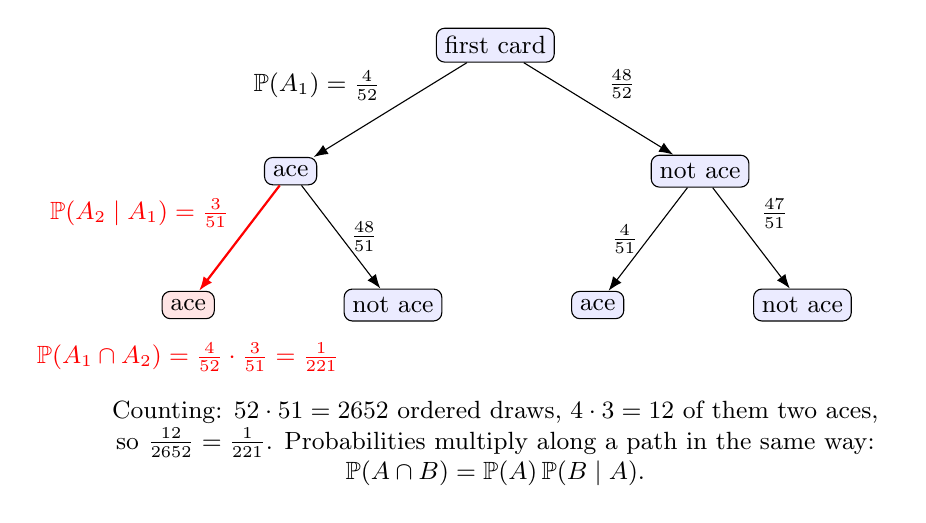
\begin{tikzpicture}[every node/.style={font=\small}, >={Latex[length=1.8mm]}, lvl/.style={draw, rounded corners=3pt, fill=blue!8, inner sep=3pt}]
	\node[lvl] (root) at (0,0) {first card};
	\node[lvl] (A) at (-2.6,-1.6) {ace};
	\node[lvl] (N) at (2.6,-1.6) {not ace};
	\draw[->] (root) -- (A) node[midway, above left, font=\small] {$\mathbb{P}(A_1)=\tfrac4{52}$};
	\draw[->] (root) -- (N) node[midway, above right, font=\small] {$\tfrac{48}{52}$};
	\node[lvl, fill=red!10] (AA) at (-3.9,-3.3) {ace};
	\node[lvl] (AN) at (-1.3,-3.3) {not ace};
	\node[lvl] (NA) at (1.3,-3.3) {ace};
	\node[lvl] (NN) at (3.9,-3.3) {not ace};
	\draw[->, red, thick] (A) -- (AA) node[midway, above left, font=\small, red] {$\mathbb{P}(A_2\mid A_1)=\tfrac3{51}$};
	\draw[->] (A) -- (AN) node[midway, right, font=\small] {$\tfrac{48}{51}$};
	\draw[->] (N) -- (NA) node[midway, left, font=\small] {$\tfrac4{51}$};
	\draw[->] (N) -- (NN) node[midway, above right, font=\small] {$\tfrac{47}{51}$};
	\node[red, anchor=north, font=\small] at (-3.9,-3.65) {$\mathbb{P}(A_1\cap A_2)=\tfrac4{52}\cdot\tfrac3{51}=\tfrac1{221}$};
	\node[anchor=north, align=flush center, text width=10cm] at (0,-4.4) {Counting: $52\cdot51=2652$ ordered draws, $4\cdot3=12$ of them two aces, so $\tfrac{12}{2652}=\tfrac1{221}$. Probabilities multiply along a path in the same way: $\mathbb{P}(A\cap B)=\mathbb{P}(A)\,\mathbb{P}(B\mid A)$.};
\end{tikzpicture}
\end{document}
